\documentclass[11pt,french]{report}
  \usepackage{babel}
  \usepackage{amsmath,amsfonts,amssymb}
  \usepackage[utf8]{inputenc}   % LaTeX
  \usepackage[T1]{fontenc}      % LaTeX
  \usepackage[autolanguage]{numprint}
  \usepackage{graphicx} %image
  	\graphicspath{{./fig/}} %fig path
  \setcounter{secnumdepth}{3} %profondeur de la numérotation du TOC
  \usepackage[colorlinks]{hyperref} %lien hypertex
  \usepackage{titlesec}	%package pour modifier les chapitres #2
  \usepackage[autolanguage]{numprint}
  \usepackage{tikz}
  \usepackage{tabularx}
  \usepackage{multirow}
  \setlength{\parindent}{0pt} %% no indent
  \frenchbsetup{StandardItemLabels=true} % pour obtenir des puces par défaut dans les listes à puces A.B.

%% set lenght figure
\setlength{\abovecaptionskip}{5pt}
%%abstract
\usepackage{epigraph}

%%maccro tikz bloc
\tikzset{
  block/.style = {draw, minimum width=5cm, minimum height=2.5cm, node distance=3cm},
  down/.style={yshift=-7em}
}

%macro position tikz
\newcommand{\tikzmark}[2]{\tikz[overlay, remember picture] \node[inner sep=0pt, outer sep=0pt, anchor=base] (#1) {#2};}


%maccro tilde
\def\utilde#1{\mathord{\vtop{\ialign{##\crcr
$\hfil\displaystyle{#1}\hfil$\crcr\noalign{\kern0.05pt\nointerlineskip}
$\hfil\tilde{}\hfil$\crcr\noalign{\kern0.05pt}}}}}


%maccro pour factoriel
\newcommand{\fact}[1]{#1\mathpunct{}!}


%% meta donnée document
\title{ACT 2003 \\ Notes de cours \\ Modèles linéaires en actuariat}
\author{\textbf{David Beauchemin}}
\date{\today}
\def\versionnumber{Automne 2017}

\usepackage{Sweave}
\begin{document}
\Sconcordance{concordance:notes_de_cours.tex:notes_de_cours.Rnw:%
1 107 1 1 0 137 1 1 22 1 2 22 1 1 9 1 2 3 1 1 6 1 2 20 1 1 14 1 2 29 1 %
1 9 1 2 42 1 1 23 1 2 194 1 1 16 1 2 13 1 1 17 1 2 129 1 1 3 2 0 1 3 1 %
0 1 3 1 0 1 3 1 0 1 3 4 0 1 2 209 1 1 15 1 2 4 1 1 5 4 0 4 1 1 3 1 0 2 %
2 3 0 1 2 13 1 1 19 1 2 1 1 1 4 7 0 1 4 7 0 1 2 218 1 1 3 2 0 1 3 1 0 1 %
1 3 0 1 2 290 1}


\makeatletter
  \begin{titlepage}
  \centering
      {\large \textbf{\textsc{UNIVERSITÉ LAVAL}}}\\
      \textsc{École d'actuariat}\\
    \vspace{2cm}
    \vspace{2cm}
      {\LARGE \textbf{\@title}} \\
    \vfill
       {\large \@author} \\
    \vspace{8cm}
        {\large\textbf{\versionnumber}}\\
    \vfill
  \end{titlepage}
\makeatother

%%%%license %%%%%
\small
{\copyright} {\the\year} David Beauchemin \\

\vspace{\baselineskip}


\includegraphics[height=7mm,keepaspectratio=true]{by-sa}\\%
Cette création est mise à disposition selon le contrat
\href{http://creativecommons.org/licenses/by-sa/4.0/deed.fr}{%
  Attribution-Partage dans les mêmes conditions 4.0 International} de
Creative Commons. En vertu de ce contrat, vous êtes libre de:
\begin{itemize}
\item \textbf{partager} --- reproduire, distribuer et communiquer
  l'{\oe}uvre;
\item \textbf{remixer} --- adapter l'{\oe}uvre;
\item utiliser cette {\oe}uvre à des fins commerciales.
\end{itemize}
Selon les conditions suivantes:

\begin{tabularx}{\linewidth}{@{}lX@{}}
  \raisebox{-9mm}[0mm][13mm]{%
    
\includegraphics[height=11mm,keepaspectratio=true]{by}} &
  \textbf{Attribution} --- Vous devez créditer l'{\oe}uvre, intégrer
  un lien vers le contrat et indiquer si des modifications ont été
  effectuées à l'{\oe}uvre. Vous devez indiquer ces informations par
  tous les moyens possibles, mais vous ne pouvez suggérer que
  l'offrant vous soutient ou soutient la façon dont vous avez utilisé
  son {\oe}uvre. \\
  \raisebox{-9mm}{
\includegraphics[height=11mm,keepaspectratio=true]{sa}}
  & \textbf{Partage dans les mêmes conditions} --- Dans le cas où vous
  modifiez, transformez ou créez à partir du matériel composant
  l'{\oe}uvre originale, vous devez diffuser l'{\oe}uvre modifiée dans
  les mêmes conditions, c'est-à-dire avec le même contrat avec lequel
  l'{\oe}uvre originale a été diffusée.
\end{tabularx}

\pagebreak

\tableofcontents

\newpage


%%%%%%% Abstract %%%%%%%
\begin{abstract}
\begin{itshape}
abstrat
\end{itshape}
\end{abstract}

%%%%%% Content %%%%%%%%

%%%%%%% Chapitre 1 %%%%%%%%
\chapter{Introduction}
L'établissement de prévisions joue un rôle central dans notre vie de tous les jours (prévisions météorologique, horoscope, etc.), et plus particulièrement dans celle des actuaires.

\subsection*{Objectifs de la régression}
Régulièrement en actuariat, on se questionne sur les effets de différentes variables sur d'autres. Par exemple,
\begin{itemize}
\item Quel est l'effet de l'âge sur la fréquence des sinistres automobiles ?
\item Quel est l'effet du sexe sur la mortalité ?
\end{itemize}

On cherche à étuider et déterminer les relations entre des variables mesurables à partir de données.

\subsection*{Deux grandes classes de variables mesurables :}
\begin{itemize}
\item Qualitatives : basées sur des opinions et/ou des intuitions.
\item Quantitatives : basées sur des observations, un modèle et des arguments mathématiques.
\end{itemize}

\subsection*{Deux \textit{grandes étapes} pour établir des prévisions quantitatives}
\begin{enumerate}
\item Bâtir le modèle et estimer les paramètres:
\begin{itemize}
\item[ex:] $F = M \times a$ Qui représente un modèle déterministe
\item[ex:] $Y =3 \times X + 6 + \epsilon_t \text{ ;où} \epsilon_t \sim N(0, 10)$ Qui représente un modèle probabiliste 
\end{itemize}
\item Calculer les prévisions à partir du modèle.
\end{enumerate}

\bigskip
Dans le cadre du cours, seulement les modèles probabilistes linéaires seront étudiez. 

%%%%%%%%%%%%%%% Chapitre 2 %%%%%%%%%%%%%%%%%%%%%%%%%%%%%
\chapter{Régression linéaire simple}

\section{Introduction}

De façon générale, en régression, nous avons :

\begin{tabularx}{\linewidth}{c|X|c}
\hline
Y & Variable dépendante, ou de réponse & Output \\
$X_1, X_2, ..., X_n$ & Soit n variables indépendantes ou explicatives, ou exogènes\footnote{Les variables $X_i$ sont indépendante par rapport à y, mais pas nécessairement entre elles.} & Input \\
$\beta_0, \beta_1, ... \beta_n$ & Les paramètres à estimer & \\
\hline
\end{tabularx}

\bigskip
\bigskip
Voici une illustration du concept de régression linéaire

%%% fig for the concept of regression operation
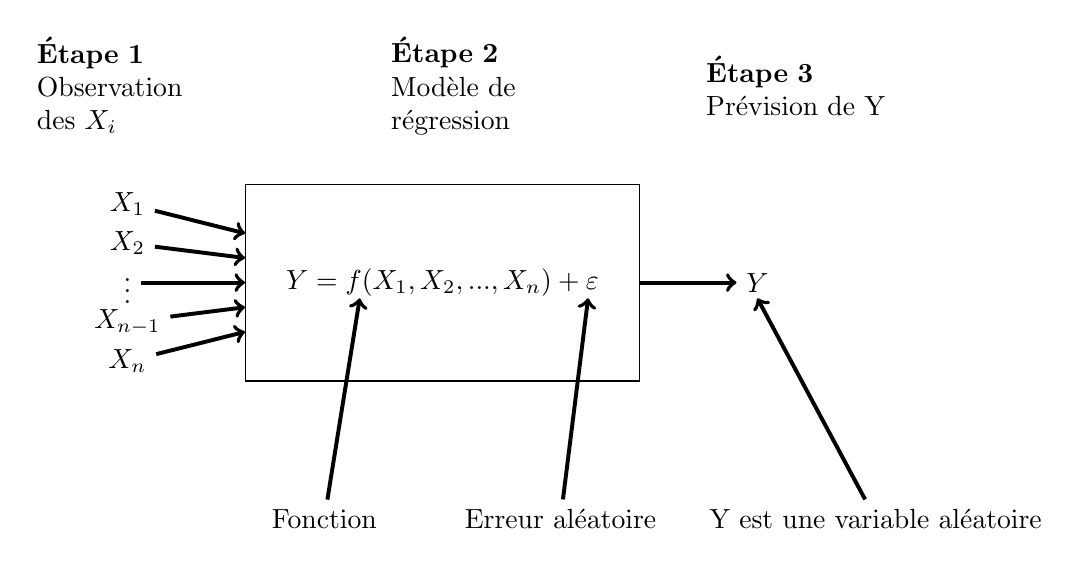
\begin{tikzpicture}
\node[block] (operator) at (4,1){$Y = f(X_1,X_2,...,X_n) + \varepsilon$};
\node[text width = 2.3cm] at (0,3.5) {\textbf{Étape 1} \\
									Observation des $X_i$};
\node[text width = 2.3cm] at (4.5,3.5) {\textbf{Étape 2} \\
									Modèle de régression};
\node[text width = 2.3cm] at (8.5,3.5) {\textbf{Étape 3} \\
									Prévision de Y};										
\node (a) at (0, 2) {$X_1$};
\draw[->, line width=0.5mm] ([right] a) --  (operator);
\node (b)at (0, 1.5) {$X_2$};
\draw[->, line width=0.5mm] ([right] b) --  (operator);
\node (c)at (0, 1) {$\vdots$};
\draw[->, line width=0.5mm] ([right] c) --  (operator);
\node (d)at (0, 0.5) {$X_{n-1}$};
\draw[->, line width=0.5mm] ([right] d) --  (operator);
\node (e)at (0, 0) {$X_{n}$};
\draw[->, line width=0.5mm] ([right] e) --  (operator);
\node (y)at (8, 1) {$Y$};
\draw[->, line width=0.5mm] (operator) -- ([left] y);
\node (F)at (2.5, -2) {Fonction};
\draw[->, line width=0.5mm] (F) --  (2.95, 0.8);
\node (E)at (5.5, -2) {Erreur aléatoire};
\draw[->, line width=0.5mm] (E) --  (5.85, 0.8);
\node (Y)at (9.5, -2) {Y est une variable aléatoire};
\draw[->, line width=0.5mm] (Y) --  (8, 0.8);
\end{tikzpicture}

\pagebreak

\subsection{Regression linéaire simple}

On cherche à prédire l'âge des passagers du Titanic selon le prix du billet à l'aide du modèle linéaire suivant,

\bigskip

%%% fig linéaire simple
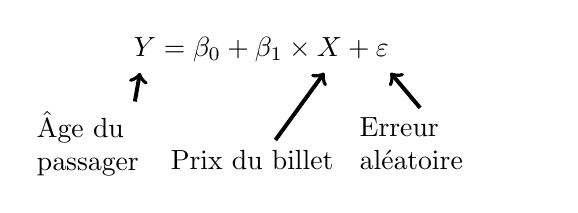
\begin{tikzpicture}[node distance=1.2cm]
\node (function) at (current page.center) {$Y  = \beta_0 + \beta_1 \times X + \varepsilon$};
\coordinate[below of=function] (c);
\node[text width = 2.3cm, left of=c, xshift=-0.5cm]  (Y) {Âge du passager};
\draw[->, line width=0.5mm] (Y) -- ([xshift=2mm, yshift=-3mm] function.west);
\node[text width = 2.3cm, below of=c, yshift=1cm] (X) {Prix du billet};
\draw[->, line width=0.5mm] (X) -- ([xshift=0.8cm, yshift=-3mm] function.center);
\node[text width = 2.3cm, right of=c, xshift=1.2cm] (E) {Erreur aléatoire};
\draw[->, line width=0.5mm] (E) -- ([xshift=-0.1cm, yshift=-3mm] function.east);
\end{tikzpicture}

%% Graphe modèle linéaire simple

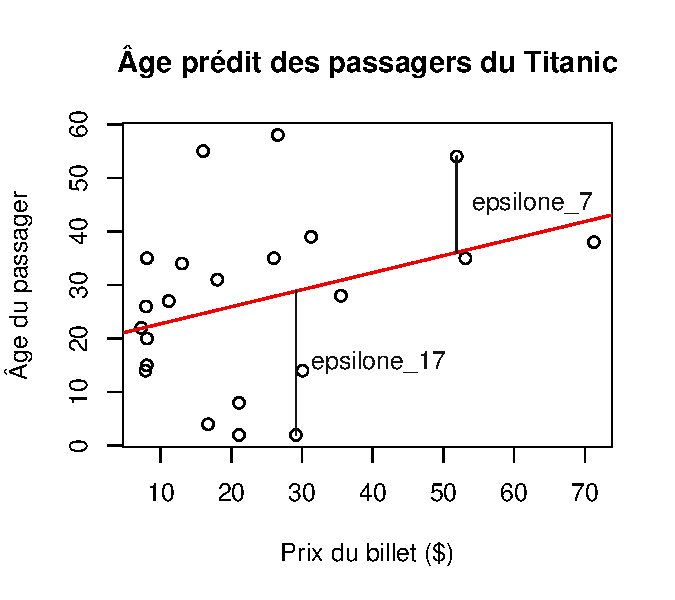
\includegraphics{notes_de_cours-001}

\subsection{Regression linéaire multiple}
On cherche à prédire l'âge des passagers du Titanic selon le prix du billet et son sexe à l'aide du modèle linéaire suivant,

\bigskip

%%% fig linéaire multiples
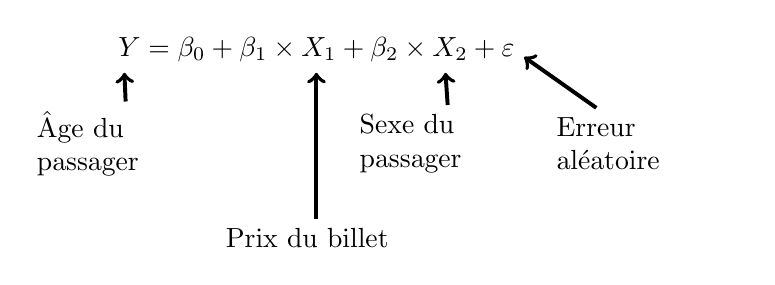
\begin{tikzpicture}[node distance=1.2cm]
\node (function) at (current page.center) {$Y  = \beta_0 + \beta_1 \times X_1 + \beta_2 \times X_2 + \varepsilon$};
\coordinate[below of=function] (c);
\node[text width = 2.3cm, left of=c, xshift=-1.2cm]  (Y) {Âge du passager};
\draw[->, line width=0.5mm] (Y) -- ([xshift=2mm, yshift=-3mm] function.west);
\node[text width = 2.3cm, below of=c, yshift=-0.0001cm] (X) {Prix du billet};
\draw[->, line width=0.5mm] (X) -- ([xshift=0cm, yshift=-3mm] function.center);
\node[text width = 2.3cm, right of=c, xshift=0.5cm] (X2) {Sexe du passager};
\draw[->, line width=0.5mm] (X2) -- ([xshift=-1cm, yshift=-3mm] function.east);
\node[text width = 2.3cm, right of=c, xshift=3cm] (E) {Erreur aléatoire};
\draw[->, line width=0.5mm] (E) -- ([ yshift=-1mm] function.east);
\end{tikzpicture}


%% fig 1 multilinear regression
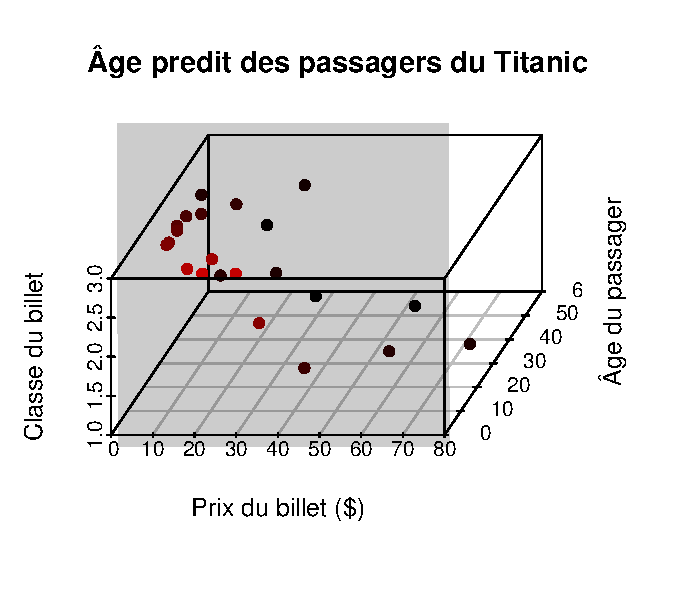
\includegraphics{notes_de_cours-002}


Voici la régression sous un autre angle, on voit la surface plane de régression.
%% fig 2
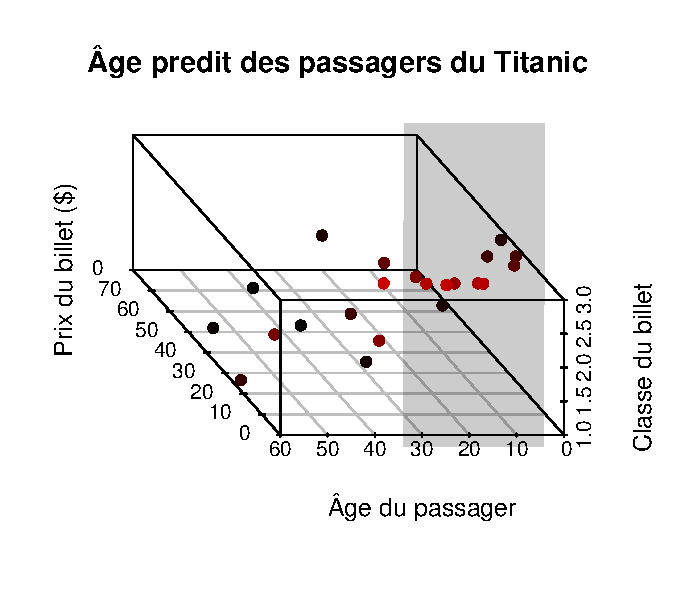
\includegraphics{notes_de_cours-003}



\subsection{Régression exponentielle}
On cherche à prédire la sévérité d'un sinistre automobile en fonction du temps à l'aide du modèle exponentielle suivant,

%%% fig exponentielle
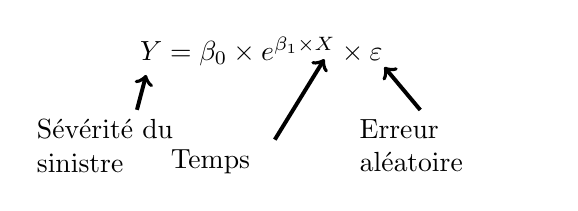
\begin{tikzpicture}[node distance=1.2cm]
\node (function) at (current page.center) {$Y  = \beta_0 \times  e^{\beta_1 \times X} \times \varepsilon$};
\coordinate[below of=function] (c);
\node[text width = 2.3cm, left of=c, xshift=-0.5cm]  (Y) {Sévérité du sinistre};
\draw[->, line width=0.5mm] (Y) -- ([xshift=2mm, yshift=-3mm] function.west);
\node[text width = 2.3cm, below of=c, yshift=1cm] (X) {Temps};
\draw[->, line width=0.5mm] (X) -- ([xshift=0.8cm, yshift=-1mm] function.center);
\node[text width = 2.3cm, right of=c, xshift=1.2cm] (E) {Erreur aléatoire};
\draw[->, line width=0.5mm] (E) -- ([xshift=-0.1cm, yshift=-2mm] function.east);
\end{tikzpicture}

%% Figure modèle exponentielle

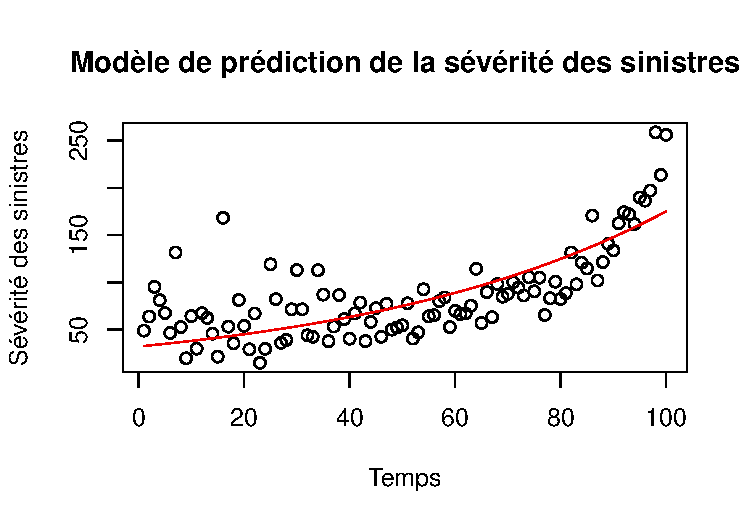
\includegraphics{notes_de_cours-004}


\subsubsection*{Note}
\label{note:exponentielle}
On remarque que la régression exponentielle est similaire à une régression linéaire simple.
\begin{align*}
\ln (Y) &= \ln (\beta_0) + \beta_1 \times X + \ln (\varepsilon) \\
Y^* &= \beta_0^* + \beta_1 \times X + \varepsilon^*\\
\end{align*}
Qu'on appel aussi une régression multiplicative ou log-linéaire.

\subsection{Régression quadratique}
On cherche à prédire la sévérité d'un sinistre automobile en fonction du temps et du temps au carré à l'aide du modèle quadratique suivant,

%%% fig quadratique
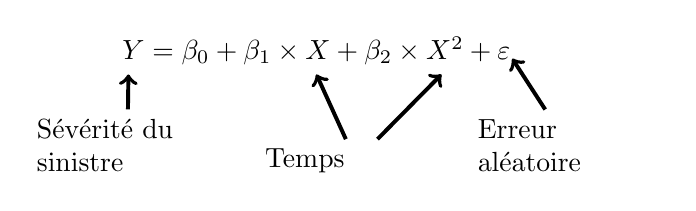
\begin{tikzpicture}[node distance=1.2cm]
\node (function) at (current page.center) {$Y  = \beta_0 + \beta_1 \times X + \beta_2 \times X^2 + \varepsilon$};
\coordinate[below of=function] (c);
\node[text width = 2.3cm, left of=c, xshift=-1.2cm]  (Y) {Sévérité du sinistre};
\draw[->, line width=0.5mm] (Y) -- ([xshift=2mm, yshift=-3mm] function.west);
\node[text width = 2.3cm, below of=c, yshift=1cm, xshift = 0.5cm] (X) {Temps};
\draw[->, line width=0.5mm] (X) -- ([xshift=0cm, yshift=-3mm] function.center);
\draw[->, line width=0.5mm] (X) -- ([xshift=-1cm, yshift=-3mm] function.east);
\node[text width = 2.3cm, right of=c, xshift=2cm] (E) {Erreur aléatoire};
\draw[->, line width=0.5mm] (E) -- ([yshift=-1mm, xshift = -1mm] function.east);
\end{tikzpicture}

%% Graphe modèle quadratique
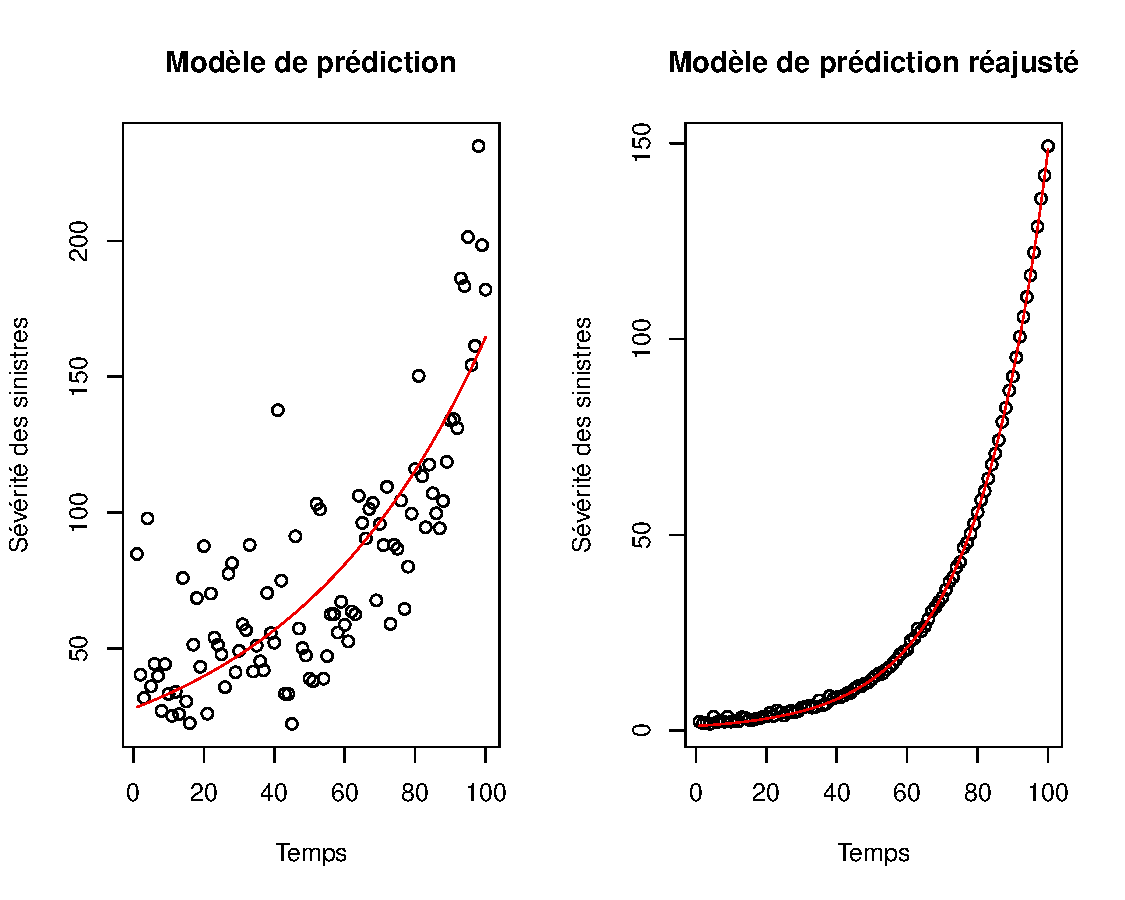
\includegraphics{notes_de_cours-005}

\subsubsection*{Note}
\label{note:quadratique}
On remarque que la régression quadratique est similaire à une régression linéaire multiple. En posant $X_1=X$ et $X_2 = X^2$
\begin{align*}
Y &= \beta_0 + \beta_1 \times X_1 + \beta_2 \times X_2 + \varepsilon\\
\end{align*}
Soit une régression linéaire multiple.

Dans le cadre du cours, seulement les modèles linéaires seront à l'étude car,

\begin{itemize}
\item Plus simples
\item Plusieurs modèles peuvent se ramener à un modèle linéaire simple ou multiple. (voir \ref{note:exponentielle} et \ref{note:quadratique})
\item Constituent souvent une très bonne approximation de la réalité qui peut être très complexe, tel que l'assurance.
\item Se généralisent faciment, tel que les \textit{Generalized Linear Models}.
\end{itemize}

Le principale problème de la modélisation linéaire est de trouver les différents paramètres $\beta_0, \beta_1, ..., \beta_n$ de tel sorte que
\begin{equation}
\varepsilon = Y - f(X_1,...,X_n; \beta_0, \beta_1,...,\beta_n)
\end{equation}
soit minimiser.


\end{document}
